\documentclass[12pt]{article}
\usepackage[margin=1in]{geometry} 		% defines page margin
\usepackage{knitting} 				% defines \chart and \textknit
\usepackage{titling} 				% title page
\usepackage{graphicx,xspace, scrextend}	% defines space control stuff
\usepackage{tabularx, array, colortbl}	% defines tables
\usepackage{multicol} 				% defines columns
\usepackage{multirow} 				% defines multirows, combined cells in tables
\usepackage{framed} 				% defines boxes for notes and written directions
\usepackage[x11names]{xcolor} 		% extends color library
\pdfmapfile{+knitfont.map}

\renewcommand{\arraystretch}{2}

\newcolumntype{L}[1]{>{\arraybackslash}p{#1}}
\newcolumntype{C}[1]{>{\centering\arraybackslash}p{#1}}

% length parameters
\setlength{\parindent}{0pt} % disables indentation for paragraphs
\setlength{\columnsep}{0.7cm} % column separation in multicol environment

% color parameters
\colorlet{framecolor}{black}
\colorlet{shadecolor}{LemonChiffon1}
\colorlet{highlight}{yellow}

% custom commands
\newcommand{\comment}[1]{} % allows for multiline comments that LaTeX will ignore

\newcommand{\vocab}[1]{\emph{\textbf{#1}}} % format for highlighting definitions of stitches, vocabulary terms
\newcommand{\rowDir}[1]{\hspace{-2em} \textbf{#1:}} % indent for written instructions within paragraphs
\newcommand{\spine}[1]{\colorbox{highlight}{#1}} % highlights spine stitches
\newcommand{\increase}[1]{(\emph{+#1 
	\ifnum#1=1{st}\else{sts}\fi})}
\newcommand{\decrease}[1]{(\emph{$-$#1
	\ifnum#1=1{st}\else{sts}\fi})}

\renewcommand{\rm}{\emph{rm}} % remove marker
\renewcommand{\pm}{\emph{pm}} % place marker

% thick horizontal line
\makeatletter \newcommand{\thickhline}{
    \noalign {\ifnum 0=`}\fi \hrule height 1.5pt
    \futurelet \reserved@a \@xhline
}
\makeatother

% custom environments
\newenvironment{frnote}
    {% framed environment for pattern notes
    	\setlength{\FrameRule}{1.5pt}
    	\def\FrameCommand{\fboxrule=\FrameRule\fboxsep=\FrameSep \fcolorbox{framecolor}{shadecolor}}
    	\MakeFramed {\FrameRestore}}
    {\setlength{\FrameRule}{1pt}
	\endMakeFramed}

\newenvironment{frdirection}
    {% framed environment for written directions
	\def\FrameCommand{\fboxrule=\FrameRule\fboxsep=\FrameSep \fbox}
   	\MakeFramed {\advance\hsize-\width \FrameRestore}
    	\addmargin[2em]{0pt}}
    {\endaddmargin
	\endMakeFramed}

\newenvironment{unframed}
    {% unframed environment for written directions
	\begin{addmargin}[1cm]{0pt}}
    {	\end{addmargin}}

\title{Mitered Nova}
\author{Shanel Wu (Piper Nell)}

\begin{document}
\begin{titlingpage}

\begin{center}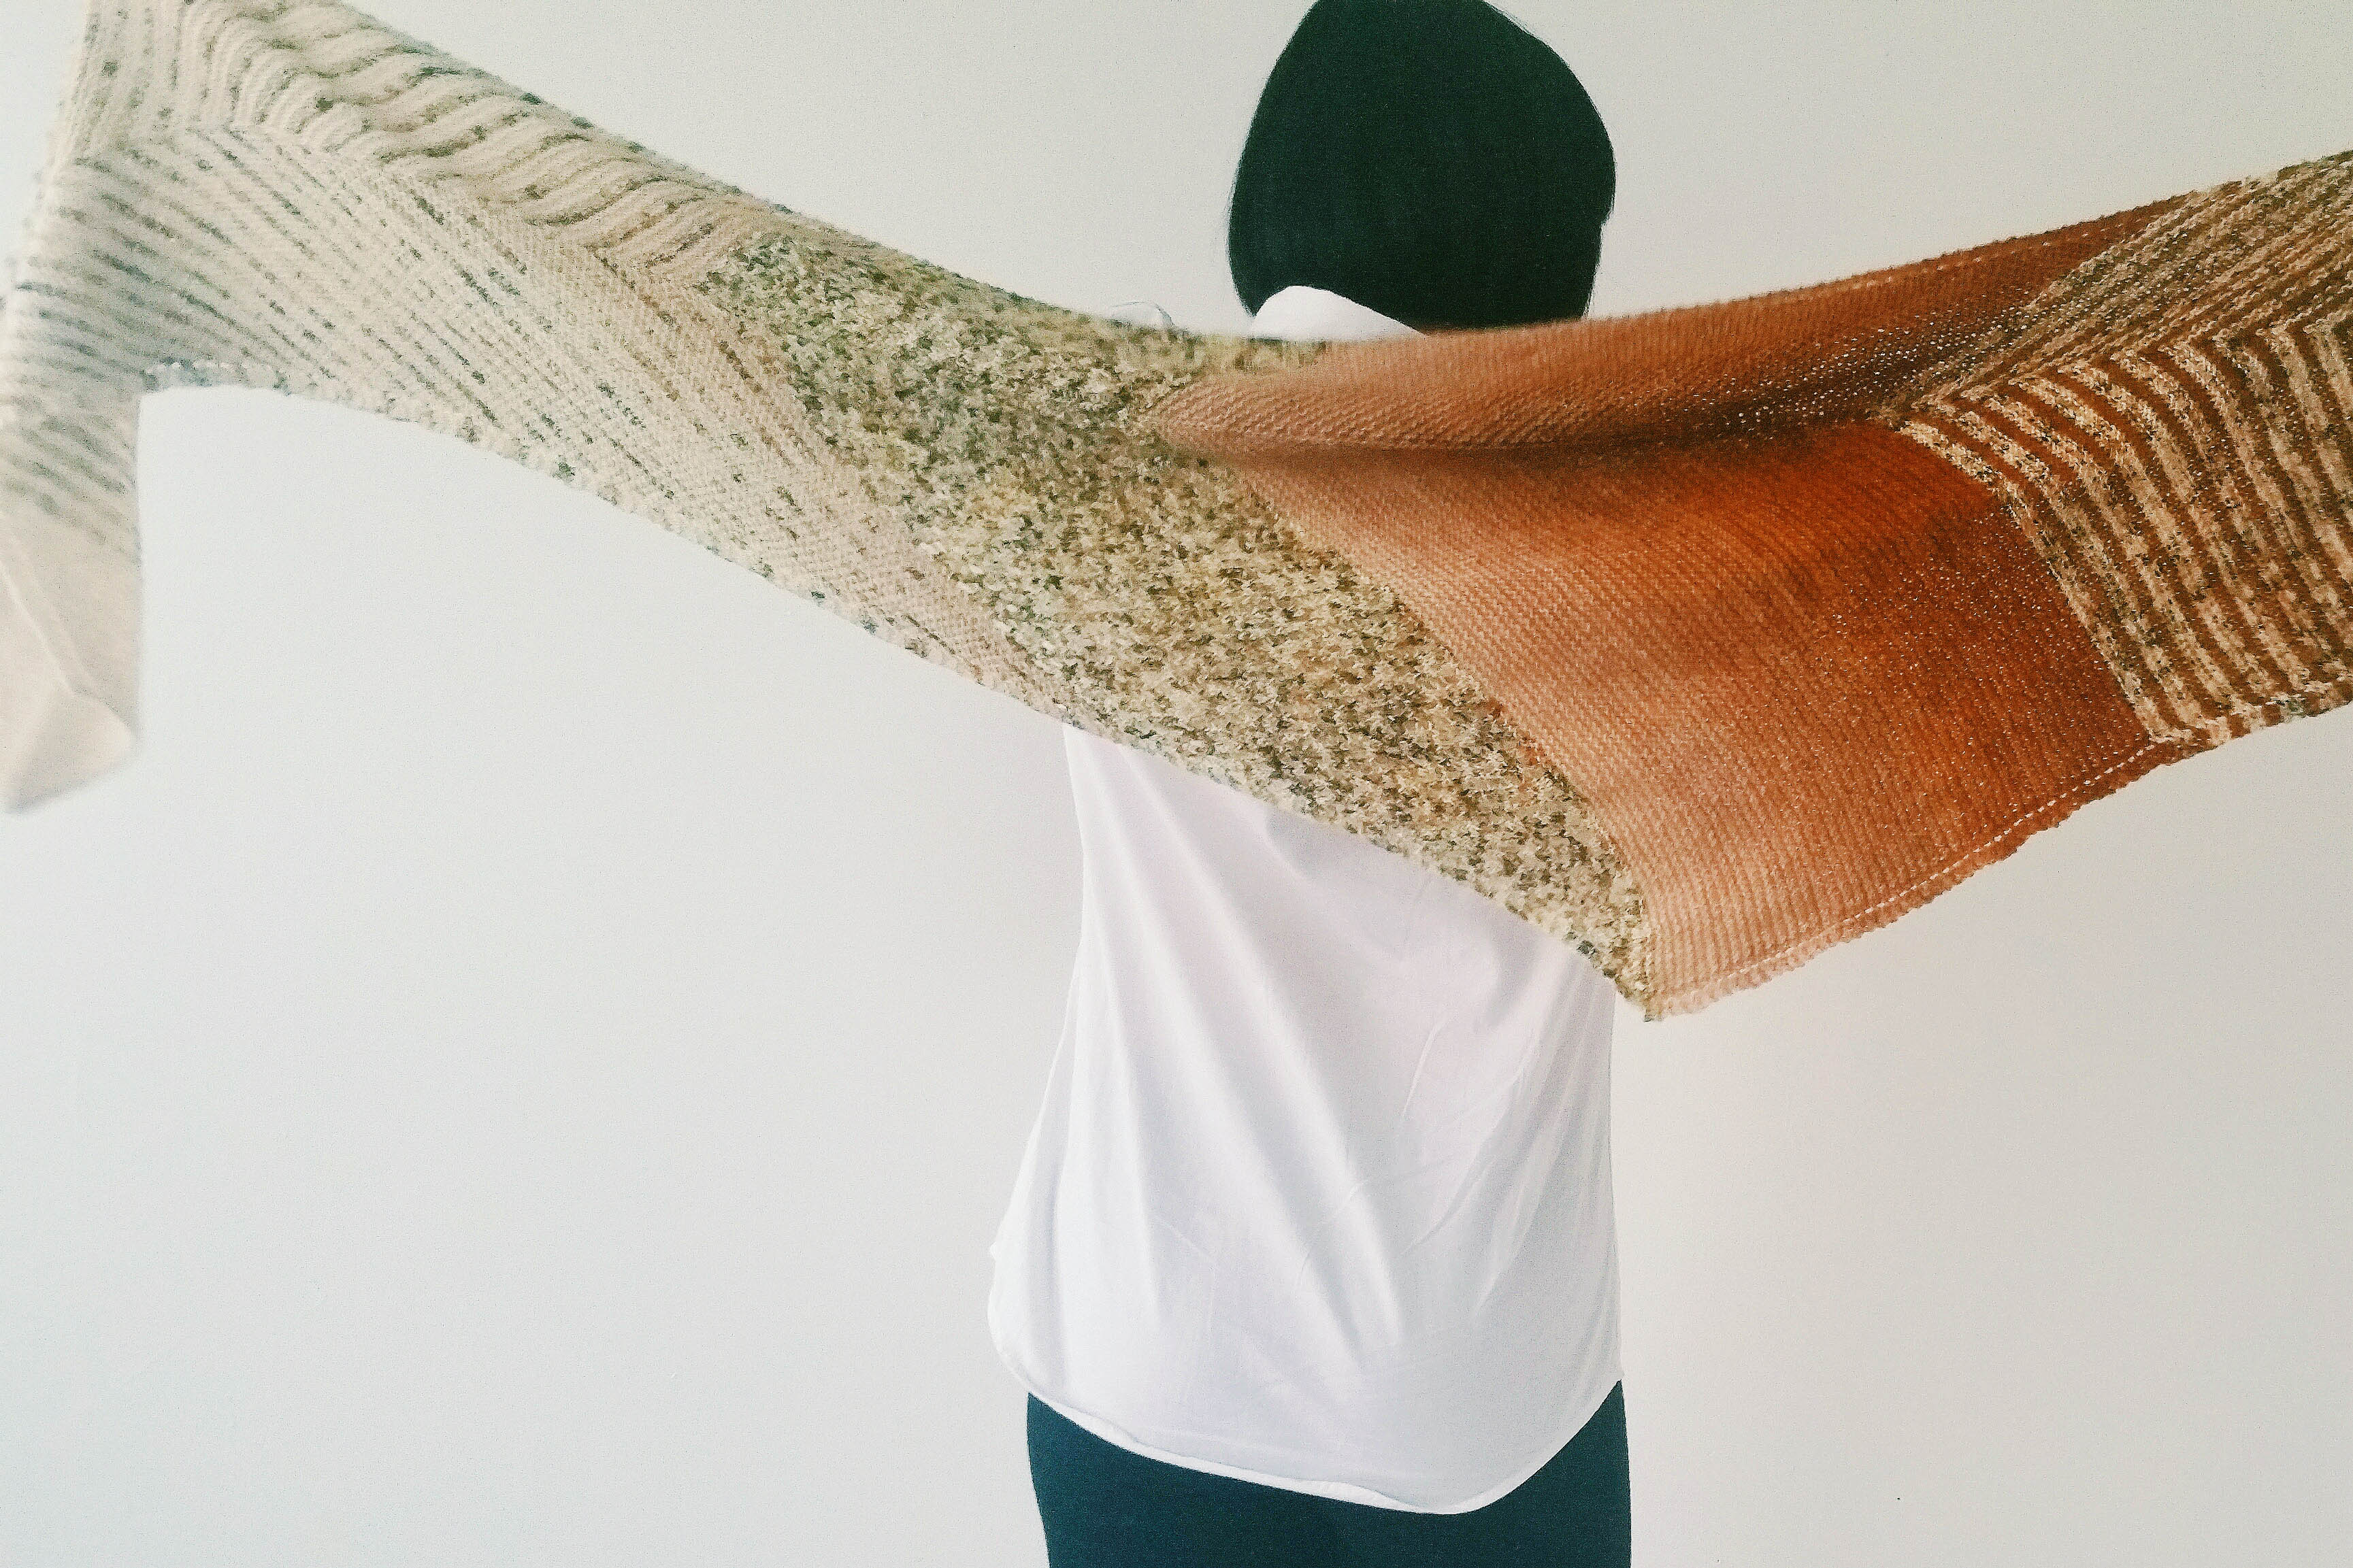
\includegraphics[width = 6.5in]{FW-spread-small} \end{center}

\begin{multicols}{2}

\section*{\thetitle}
\vspace{-1em}
\subsubsection*{\theauthor}
\subsubsection*{Materials}

You'll need two colors (C1 and C2) and a long (at least 32") circular needle. \\ Yardage, sample gauge, and recommended needle sizes are in the table that follows. Gauge is not important, but may affect yarn consumption and final size of the piece.

\vfill
\columnbreak
\subsubsection*{Notions}
\begin{itemize}
\item Tapestry needle \vspace{-1em}
\item Removable stitch markers (optional)
\end{itemize}

\vspace{-1em}

\subsubsection*{Reading}

One set of directions is given for both versions of the shawl, lace weight and fingering weight. Repeat and stitch counts differ by yarn weight and are given in the format \mbox{\vocab{lace(fingering)}. [e.g. knit 45(35) sts]} 
\end{multicols}

\vfill
% materials table w/ yardage and needle size for two versions
\begin{tabular}{ | C{0.15\linewidth}  C{0.4\linewidth}  C{0.4\linewidth} |}
\thickhline \rowcolor{shadecolor}
{} 			&\textbf{Lace weight} 	& \textbf{Fingering weight} \\ \thickhline
\textbf{Yardage}	& C1: 75g/645y, C2: 50g/400y		& C1: 100g/420y, C2: 100g/420y \\
\textbf{Gauge}	& {26 st x 46 rows/4"(10cm)}	& {23 st x 40 rows/4"(10cm)} \\ 
\textbf{Needle} \mbox{(32" or longer)}	& US3 (2.75mm)		& US5 (3.75mm) \\ \hline
\end{tabular}

\newpage

%%%%%%%%%%%%%%%%%%%%%%%%%%%%%%%%%%%%%%%%
\subsection*{Pattern Key}

Pattern repeats will be indicated with thick borders (chart) or asterisks \textbf{*[stitches]*} (written). Spine stitches will be \spine{highlighted}. All odd-numbered rows will be on the right side of the work (RS) and all even-numbered rows will be on the wrong side (WS).
\vspace{-1em}
\begin{center}
\begin{tabular}{| C{0.15\linewidth}  C{0.2\linewidth}  p{0.6\linewidth} | }
\thickhline \rowcolor{shadecolor} 
\textbf{Chart}	& \textbf{Written}	& \textbf{Name \& Description} \\ \thickhline
\chart{-}	& k (RS); p (WS)	&  knit (RS); purl (WS)	\\
\chart{=} 	& p (RS); k (WS)	& purl  (RS); knit (WS) \\
N/A		& s1 wyib		& slip one stitch with yarn in back \\
\chart{kK} 	& r2t		& right twist or right mini-cable \emph{(See appendices.)}\\
\chart{Kk}	& l2t		& left twist or left mini-cable \emph{(See appendices.)} \\  
\multicolumn{3}{| c |}{\cellcolor{shadecolor}\textbf{increases}} \\ 
\chart{O} 	& yo		& yarn-over  \\
\chart{v}	& kfb		& \textbf{knit front back:} knit stitch through front loop, then in the same stitch, knit through the back loop; single increase		\\
\chart{w}	& kyok	& \textbf{knit yarn-over knit:} in a single stitch, knit, yarn over, then knit again; double increase		\\ 
\multicolumn{3}{| c |}{\cellcolor{shadecolor} \textbf{decreases}} \\ \
\chart{>}	& k2tog 	& \textbf{knit 2 together:} single decrease, right-leaning \\
\chart{<}	& ssk		& \textbf{slip slip knit:} single decrease, left-leaning \\
\chart{A} 	& cdd		& \textbf{central double-decrease:} slip two stitches as if to k2tog, k next stitch, pass 2 slipped st over \\
\chart{R}	& k3tog 	& \textbf{knit 3 together:} double decrease, right-leaning \\
\chart{L}	& sssk		& \textbf{slip slip slip knit:} slip 3 knitwise individually, k3tog through back loop; double decrease, left-leaning \\
\hline
\end{tabular}
\end{center}

\end{titlingpage}
%%%%%%%%%%%%%%%%%%%%%%%%%%%%%%%%%%%%%%%%
\newpage
\begin{multicols}{2}
\section*{S1: Steady State}

\begin{unframed}
\rowDir{Cast On} With C1, CO 91 (71) stitches using the long-tail cast on. \\ The middle stitch, the 46th (36th) stitch, will be referred to as the \vocab{spine stitch} or the \vocab{spine} and will be \spine{highlighted} when appropriate. On every RS row, the spine stitch will be the center stitch in a centered double-decrease (cdd). On every WS row, the spine stitch will be purled.
 
\rowDir{Set-up row} (WS) k 45 (35) sts, \spine{p1}, k to end. 
\end{unframed}

Next, work 25 (20) repeats of Rows 1-2 as follows, for a total of 50 (40) rows. Each repeat forms a \vocab{straight ridge} in garter stitch.

\begin{frdirection}
\rowDir{Row 1} (RS) k3, yo, k to 1 st before spine, \spine{cdd},  k to 3 sts before end, yo, k3.

\rowDir{Row 2} (WS) k to spine, \spine{p1}, k to end.
\end{frdirection}

You should end Section 1 with the same number of stitches as you started, 91 (71) sts.

%%%%%%%%%%%%%%%%%%%%%%%%%%%%%%%%%%%%%%%%
\section*{S2: Expanding Stripes}
\begin{unframed}
\rowDir{Set-up stripe (6 rows)} Switch to C2 and work one \textbf{straight ridge}. Then switch back to C1, carrying C2 up the edge, and work two more \textbf{straight ridges}. 
\end{unframed}

Next, work 30 (20) repeats of Rows 1-6 as follows. Each 6-row repeat forms one \vocab{increase stripe}, consisting of one \textbf{increase ridge} in C2 (Rows 1-2) then two \textbf{straight ridges} in C1, increasing by 1 st per repeat. 

\begin{frdirection}
\rowDir{Row 1} (C2) k3, yo, k to 1 st before spine, \spine{cdd}, k to 3 sts before end, yo, k3.

\rowDir{Row 2} (C2) k to spine, \spine{p1}, k to 4 sts from end, kfb, k3. \increase{1}
\\ (\emph{Rows 1-2 form an \textbf{increase ridge}})

\rowDir{Row 3} (C1) Repeat Row 1.

\rowDir{Row 4} (C1) k to spine, \spine{p1}, k to end.

\rowDir{Row 5 \& 6} (C1) Repeat Rows 3 \& 4.
\end{frdirection}

At the end of Section 2, you should have 121 (91) sts. 

\begin{frnote}
\textbf{Stitch markers:} Some test knitters found that marking the spine with a stitch marker helped them read their work. Experiment with different marker placements to see what helps you!
\end{frnote}

%%%%%%%%%%%%%%%%%%%%%%%%%%%%%%%%%%%%%%%%
\section*{S3: Lace Nova}
Lace instructions are both written and charted according to the pattern key. The main lace motif is a 5-stitch, 6-row repeat where all wrong side sts (minus edge stitches) are purled. WS rows after Row 2 are omitted in the written instructions. Increases are worked into yo of previous row. Each repeat of \textbf{Chart A} increases by 5 sts.

\begin{unframed} \rowDir{Set-up (2 rows)} Break C1, switch to C2, and work one \textbf{straight ridge} as follows: \end{unframed}
\begin{frdirection}
\rowDir{Row 1} (RS) k3, yo, k to 1 st before spine, \spine{cdd},  k to 3 sts from end, yo, k3.

\rowDir{Row 2} (WS) k to spine, \spine{p1}, k to end.
\end{frdirection}

Next, work 8 (8) repeats of \textbf{Chart A}. \vspace{-1em}

\newpage
\end{multicols}

\subsection*{Chart A}

\chart{
\rnleft ===\!\overline{-----}\!--\spine{-}--\!\overline*{-----}\!-------w===
---\!OLO--\!O-\spine{A}-O\!--ORO\!--ORO--O--- \rnright
\rnleft ===\!-----\!--\spine{-}--\!-----\!-----v===
---\!O<Kk-\!O-\spine{A}-O\!-kK>O\!-kK>-O--- \rnright
\rnleft ===\!-----\!--\spine{-}--\!-----\!----v===
---\!\underline*{O<-Kk}\!O-\spine{A}-O\!\underline*{kK->O}\!kK->O---		\rnright
}

\vspace{1em}
\begin{multicols}{2}

\subsection*{Chart A (written)}
\begin{unframed} 
\rowDir{Row 1} k3, yo, k2tog, k1, r2t, \textbf{*[yo, k2tog, k1, r2t]*} to 2 sts before spine, \\ yo, k1, \spine{cdd}, k1, yo, \textbf{*[l2t, k1, ssk, yo]*} to 3 sts from end, k3

\rowDir{Row 2} k3, p to 4 sts from end, kfb, k3 \increase{1}

\rowDir{Row 3} k3, yo, k1, k2tog, r2t, k1, \textbf{*[yo, k2tog, r2t, k1]*} to 2 sts before spine, \\ yo, k1, \spine{cdd}, k1, yo, \textbf{*[k1, l2t, ssk, yo]*} to 3 sts from end, k3

\rowDir{Row 4} Repeat Row 2. \increase{1}

\rowDir{Row 5} k3, yo, k2, yo, k3tog, yo, k2, \textbf{*[yo, k3tog, yo, k2]*} to 2 sts before spine, \\ yo, k1, \spine{cdd}, k1, yo, \textbf{*[k2, yo, sssk, yo]*} to 3 sts from end, k3 \increase{1}

\rowDir{Row 6} k3, p to 4 sts from end, kyok, k3 \increase{2}
\end{unframed}

After the last lace repeat, work one more \textbf{straight ridge} before moving onto the next section. At the end of Section 3, you should have 161 (131) sts.

\section*{S4: Contracting}
Break C2 and switch to C1. Work 40 (30) repeats of Rows 1-2 as follows. Each repeat decreases 1 st and forms a \vocab{decrease ridge}.

\begin{frdirection}
\rowDir{Row 1} k3, yo, k to 1 st before spine, \spine{cdd}, k to 3 sts from end, yo, k3.

\rowDir{Row 2} k to spine, \spine{p1}, k to 6 sts from end, k2tog, k4. \decrease{1}
\end{frdirection}

At the end of Section 4, you should have 121 (101) sts on your needles.

\vfill
\columnbreak

%%%%%%%%%%%%%%%%%%%%%%%%%%%%%%%%%%%%%%%%

\section*{S5: Contracting Stripes}
Rejoin C2. Work 15 (15) repeats of Rows 1-6 as follows, decreasing while striping C1 and C2. Each 6-row repeat forms one \vocab{decrease stripe}, consisting of two \textbf{decrease ridges} in C2 followed by one \textbf{straight ridge} in C1, decreasing by 2 sts per repeat.

\begin{frdirection}
\rowDir{Row 1} (C2) k3, yo, k to 1 st before spine, \spine{cdd}, k to 3 sts from end, yo, k3.

\rowDir{Row 2} (C2) k to spine, \spine{p1}, k to 6 sts from end, k2tog, k4. \decrease{1}

\rowDir{Rows 3 \& 4} (C2) Repeat Rows 1 \& 2. \decrease{1}

\rowDir{Row 5} (C1) Repeat Row 1.

\rowDir{Row 6} (C1) k to spine, \spine{p1}, k to end.
\end{frdirection}

At the end of Section 5, you should have your original stitch count, 91 (71) sts.
\end{multicols}

%%%%%%%%%%%%%%%%%%%%%%%%%%%%%%%%%%%%%%%%
\newpage
\subsection*{Chart B}

\chart{
\rnleft ===\!\overline{-----}\!--\spine{-}--\!\overline*{-----}\!=== 
---\!OLO--\!O-\spine{A}-O\!--ORO\!--- \rnright
\rnleft ===\!-----\!--\spine{-}--\!-----\!===
---\!O<Kk-\!O-\spine{A}-O\!-kK>O\!--- \rnright
\rnleft ===\!-----\!--\spine{-}--\!-----\!===
---\!\underline*{O<-Kk}\!O-\spine{A}-O\!\underline*{kK->O}\!--- \rnright
}

\vspace{1em}

\begin{multicols}{2}

\section*{S6: Lace Steady State}
\begin{unframed} \rowDir{Set-up (2 rows)} Break C1, switch to C2, and work one \textbf{straight ridge}. \end{unframed}

\begin{frdirection}
\rowDir{Row 1} (RS) k3, yo, k to 1 st before spine, \spine{cdd},  k to 3 sts before end, yo, k3.

\rowDir{Row 2} (WS) k to spine, \spine{p1}, k to end.
\end{frdirection}

Next, work 8 (10) repeats of \textbf{Chart B}. 

\subsection*{Chart B (written)}

\begin{unframed}
\rowDir{Row 1} k3, \textbf{*[yo, k2tog, k1, r2t]*} to 2 sts before spine, yo, k1, \spine{cdd}, k1, yo, \textbf{*[l2t, k1, ssk, yo*]} to 3 sts from end, k3 

\rowDir{Row 2} k3, p to 3 sts from end, k3 \emph{(all WS rows are identical to Row 2)}

\rowDir{Row 3} k3, \textbf{*[yo, k2tog, r2t, k1]*} to 2 sts before spine, yo, k1, \spine{cdd}, k1, yo, \textbf{*[k1, l2t, ssk, yo]*} to 3 sts from end, k3

\rowDir{Row 5} k3, \textbf{*[yo, k3tog, yo, k2]*} to 2 sts before spine, yo, k1, \spine{cdd}, k1, yo, \textbf{*[k2, yo, sssk, yo]*} to 3 sts from end, k3
\end{unframed}

After the last lace repeat, work one more \textbf{straight ridge} before moving on. You should end Section 6 with the same number of stitches as you started, 91 (71) sts.

\vfill
\columnbreak
%%%%%%%%%%%%%%%%%%%%%%%%%%%%%%%%%%%%%%%%

\section*{S7: Mitered Square}

Break C2 and switch to C1 for this last section. Work a mitered square by repeating the following two rows:

\begin{unframed}
\rowDir{Row 1} (RS) slip 1 with yarn in back (\textbf{s1 wyib}), k to 1 before spine, \spine{cdd}, k to end

\rowDir{Row 2} (WS) s1 wyib, k to spine, \spine{p1}, k to end
\end{unframed}

Each repeat decreases by 2 sts. Repeat Rows 1 and 2 until 5 sts are left at the end of a WS row. 

Work the last 3 rows as follows:

\begin{unframed}
\rowDir{Row 1} (RS) s1 wyib, cdd, k1 (3 sts)

\rowDir{Row 2} (WS) k1, p1, k1 (3 sts)

\rowDir{Row 3} (RS) cdd (1 st)
\end{unframed}

Break yarn, leaving a 6 inch tail. Pull the loop of the last stitch through to finish. 

\begin{frnote}
\textbf{Finishing:} Block the piece, weave in all ends, and enjoy your new shawl! I would recommend blocking wires for the edges. I also suggest pinning down the spine as you block to help shape the shawl.
\end{frnote}
\end{multicols}



\end{document}